\section{Studies of effective jet radius}
\label{sec:jets}


The effective radius is the average of the energy weighted radial distance in $\eta-\phi$ space of jet constituents.
Recently, it has been studied for multi-TeV jets in Ref.\cite{Auerbach:2014xua}.
 

\begin{figure}
\begin{center}
   \subfigure[5 TeV] {
   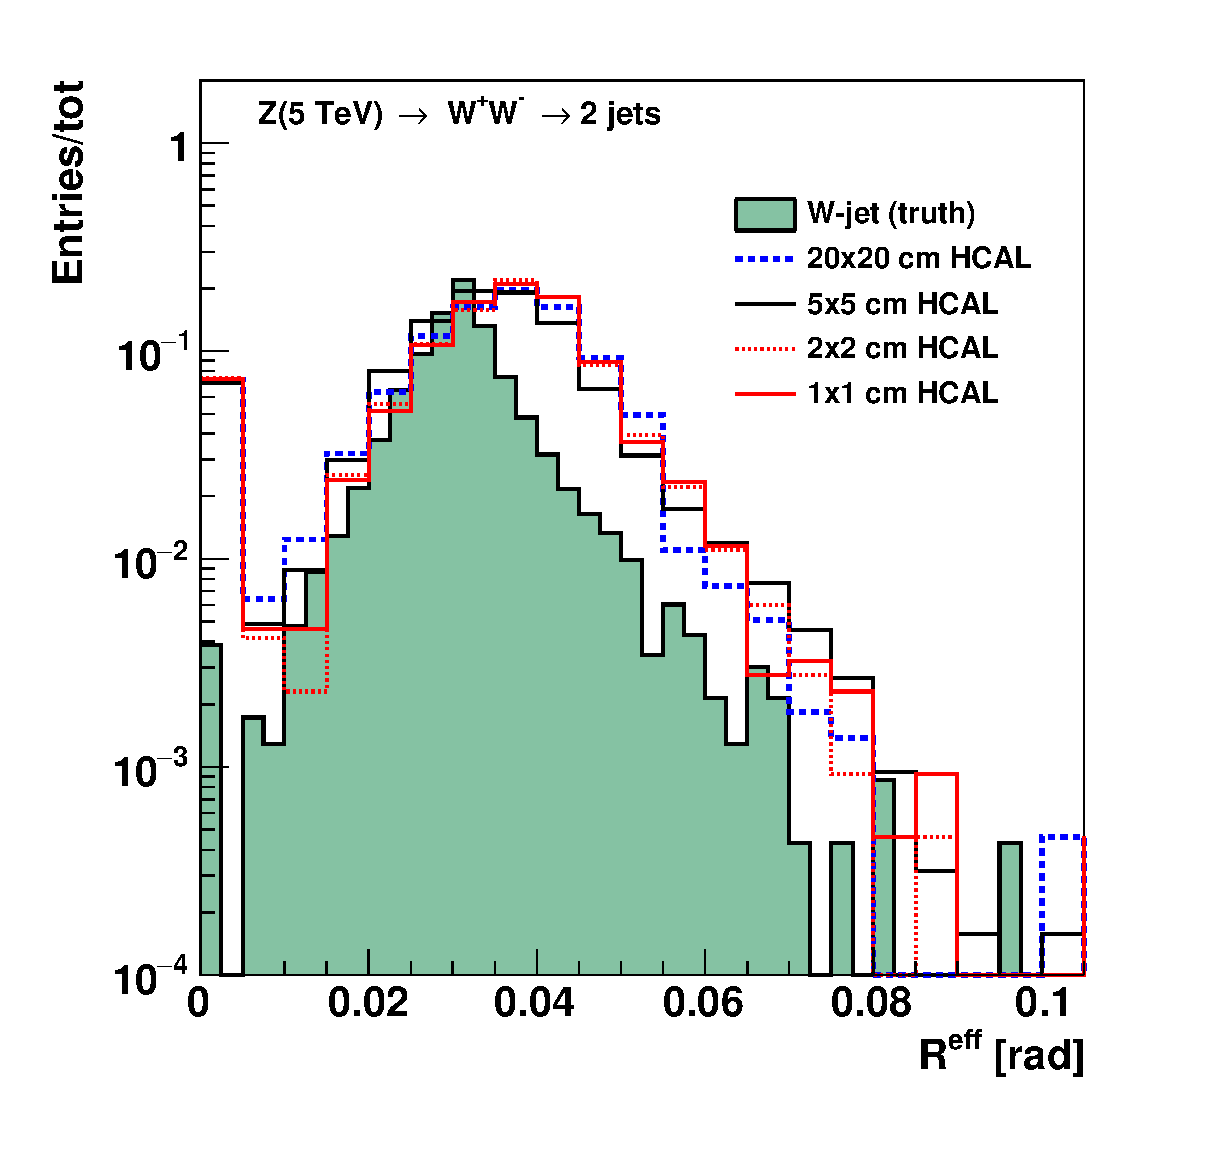
\includegraphics[width=0.43\textwidth]{figs/h5tev_clus_effR_ww1}\hfill
   }
   \subfigure[10 TeV] {
   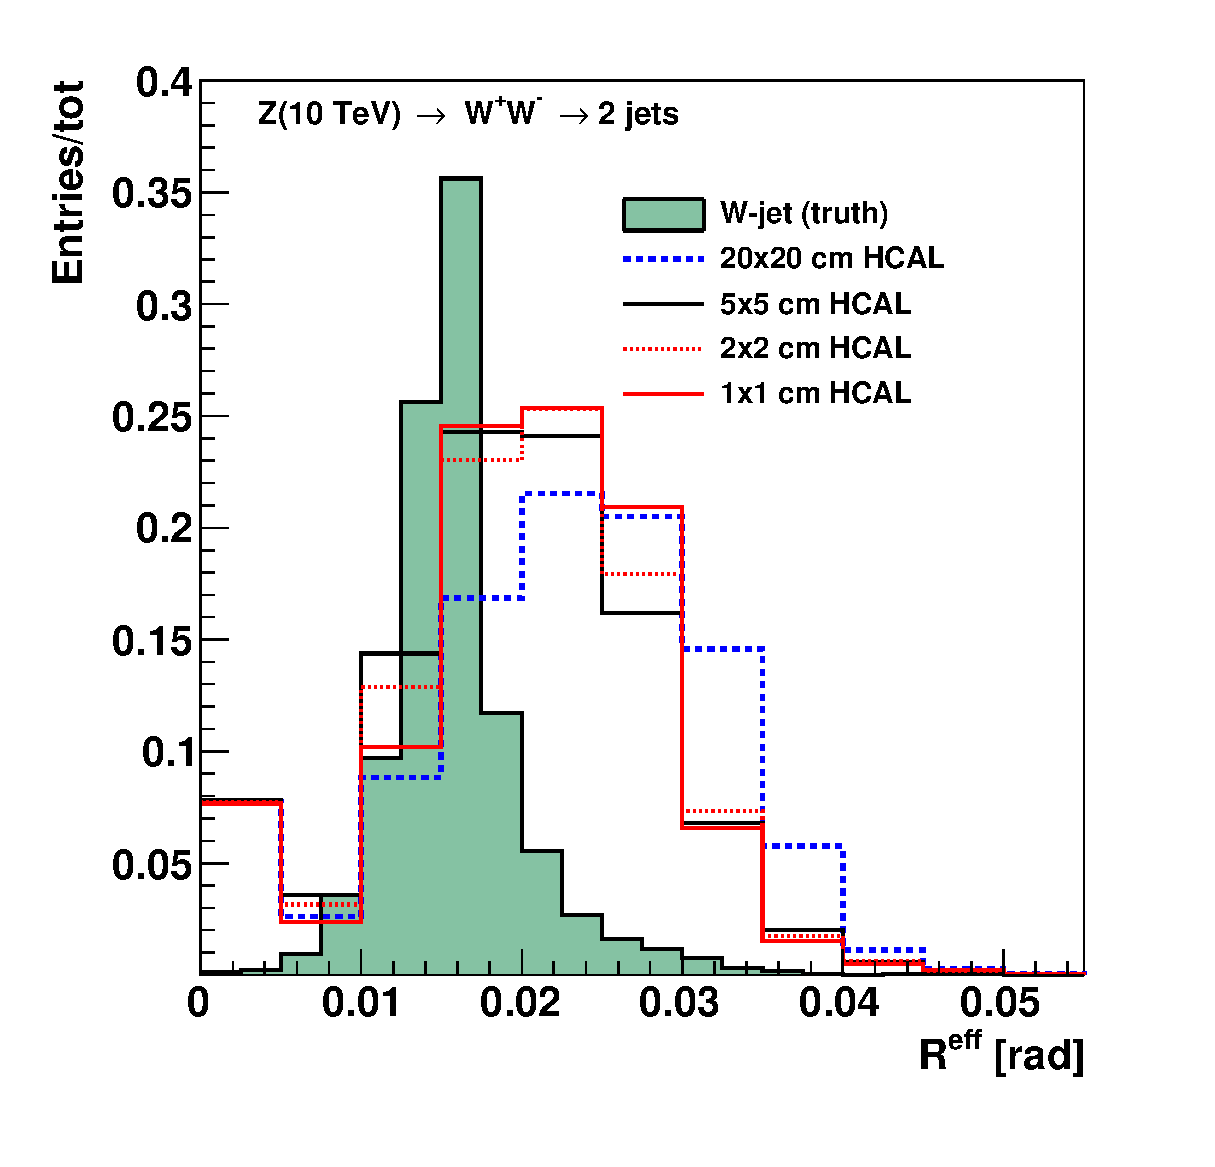
\includegraphics[width=0.43\textwidth]{figs/h10tev_clus_effR_ww1}
   }
   \subfigure[20 TeV] {
   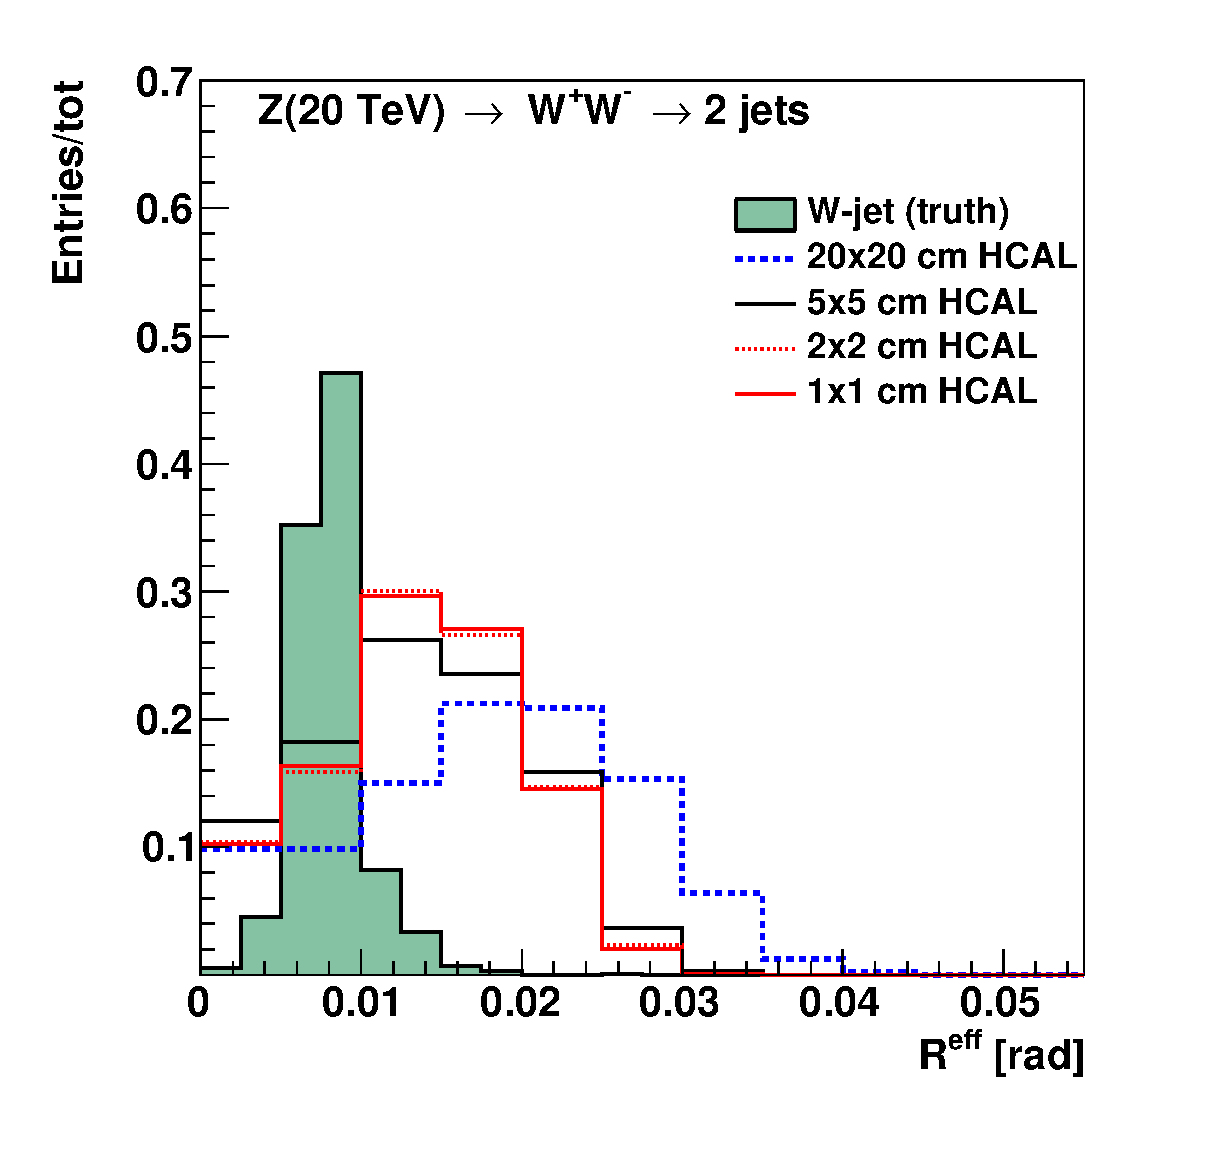
\includegraphics[width=0.43\textwidth]{figs/h20tev_clus_effR_ww1}
   }
   \subfigure[40 TeV] {
   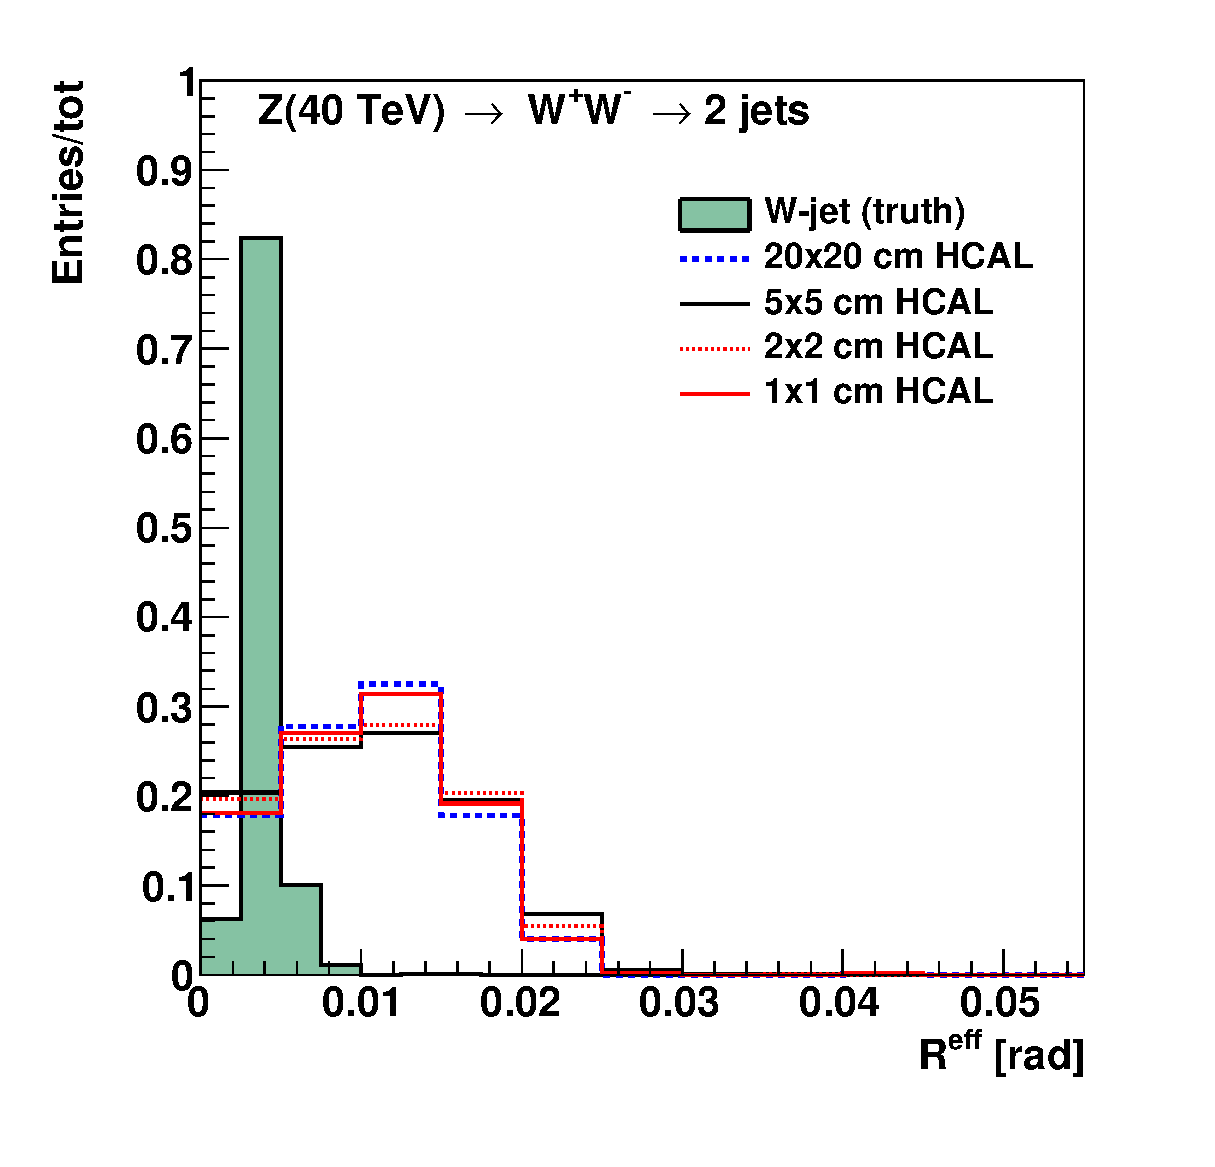
\includegraphics[width=0.43\textwidth]{figs/h40tev_clus_effR_ww1}
   }
\end{center}
\caption{Jet effective radius for different jet transverse moment and HCAL granularity.}
\label{fig:eff_rad}
\end{figure}


New we sill study jet splitting the effect of granularity on jet splitting scales.
A jet $k_T$ splitting scale \cite{Butterworth:2002tt} is defined as a distance measure
used to form jets by the $k_T$ recombination
algorithm \cite{Catani1993187,Ellis:1993tq}.
This has been studied by ATLAS~\cite{ATLAS:2012am}, and more recently in the context of 100 TeV physics \cite{Auerbach:2014xua}.
The distribution of the splitting scale $\sqrt{d_{12}}=\min(p_T^1,p_T^2) \times \delta R_{12}$ \cite{ATLAS:2012am} at the final stage of the $k_T$ clustering, where two subjets are merged into the final one,
is shown in Fig.~\ref{fig:d12}.

\begin{figure}
\begin{center}
   \subfigure[5 TeV] {
   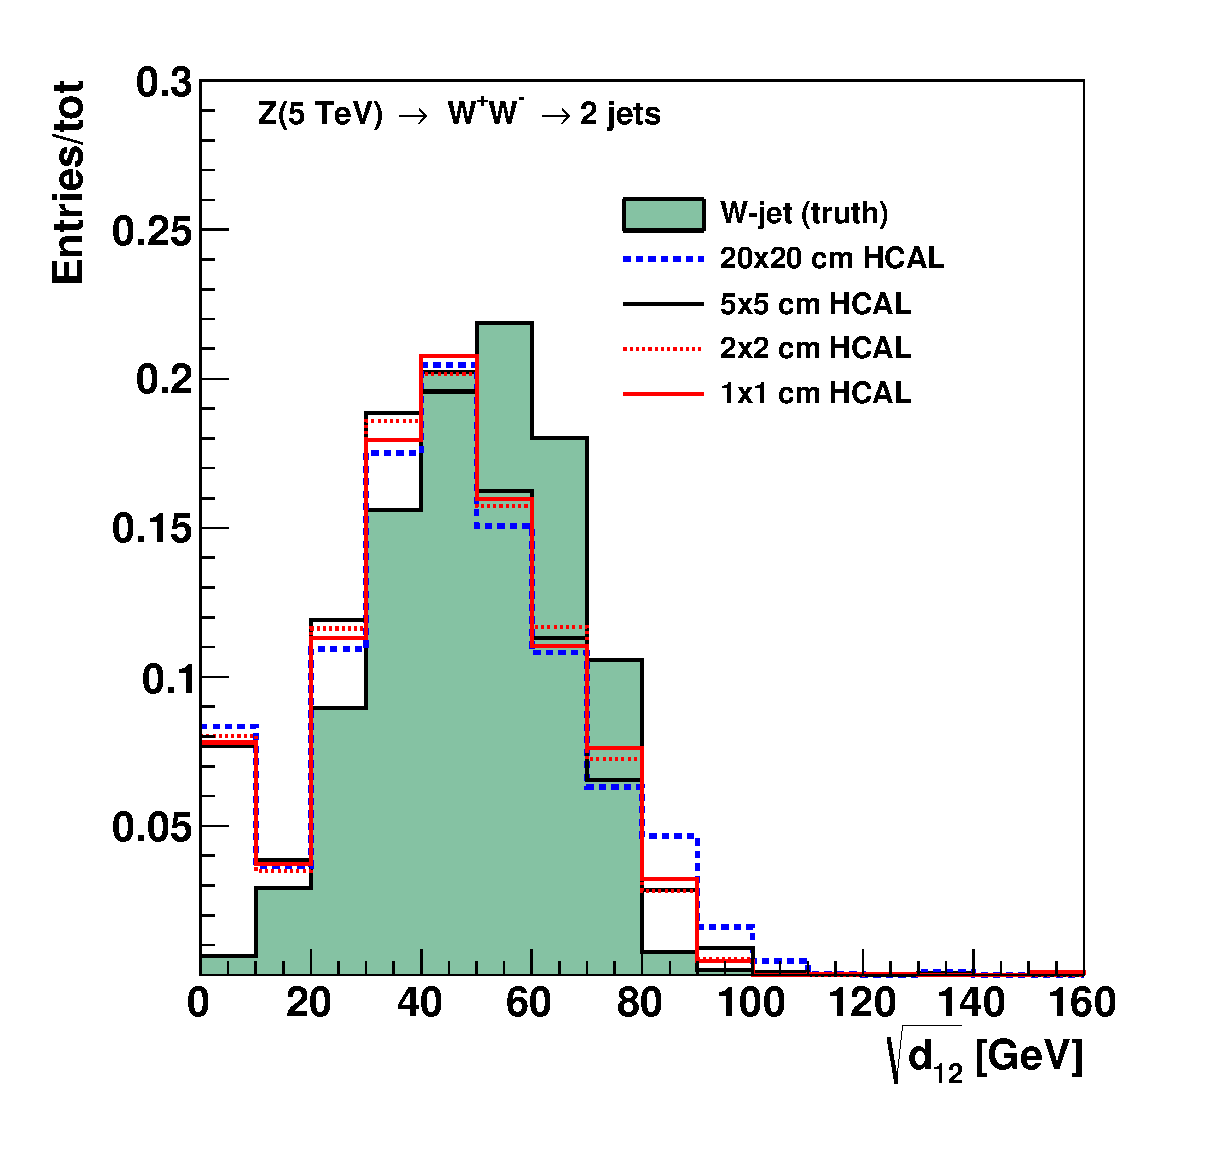
\includegraphics[width=0.43\textwidth]{figs/h5tev_clus_d12_ww1}\hfill
   }
   \subfigure[10 TeV] {
   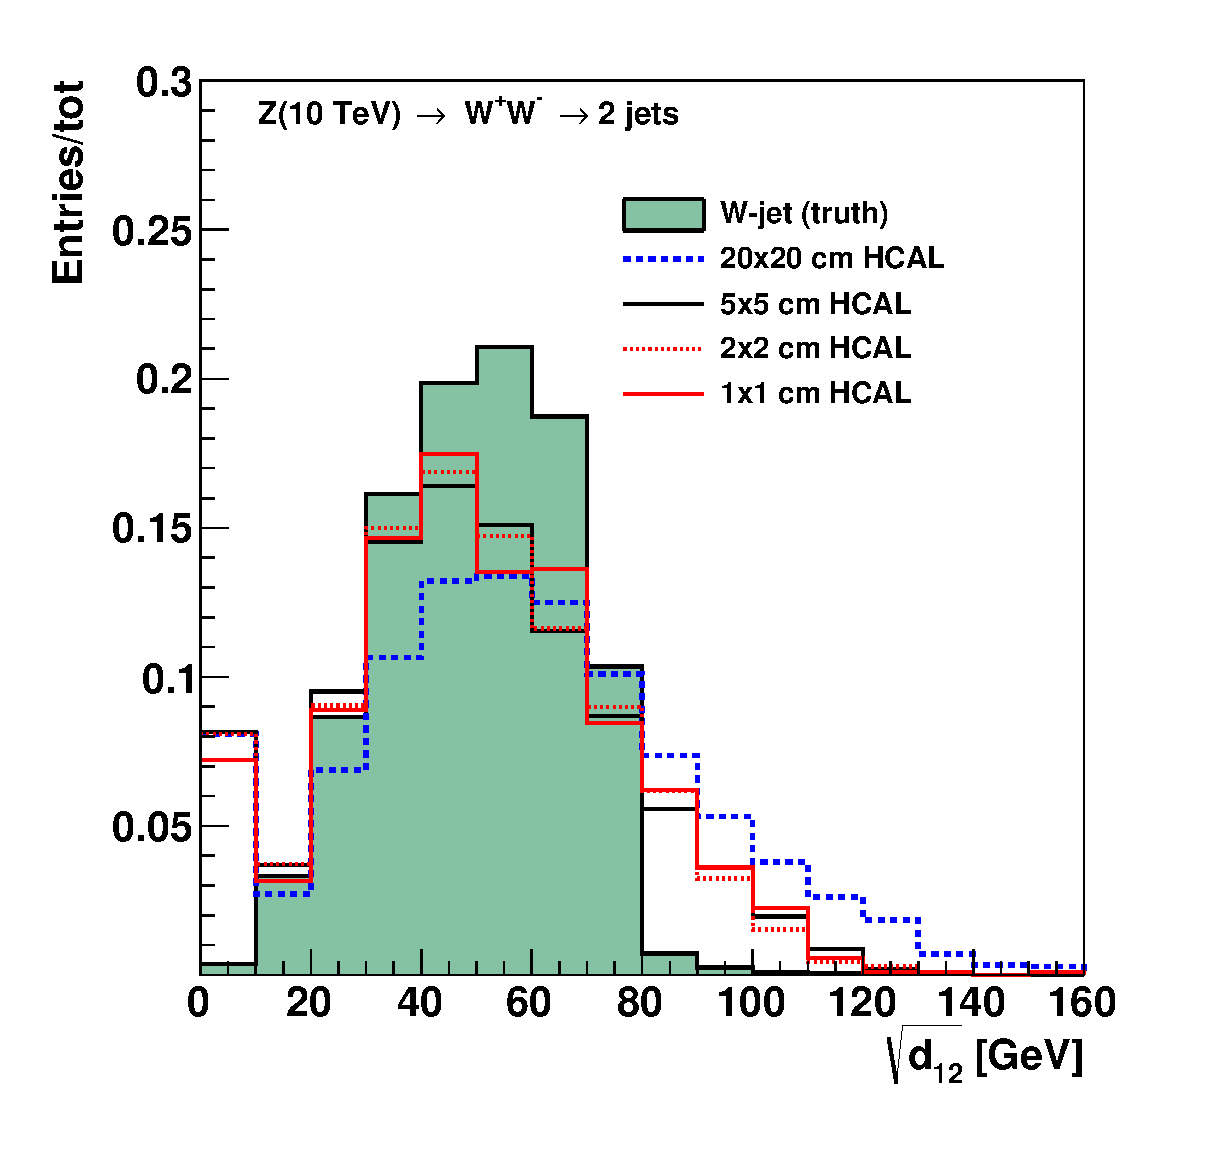
\includegraphics[width=0.43\textwidth]{figs/h10tev_clus_d12_ww1}
   }
   \subfigure[20 TeV] {
   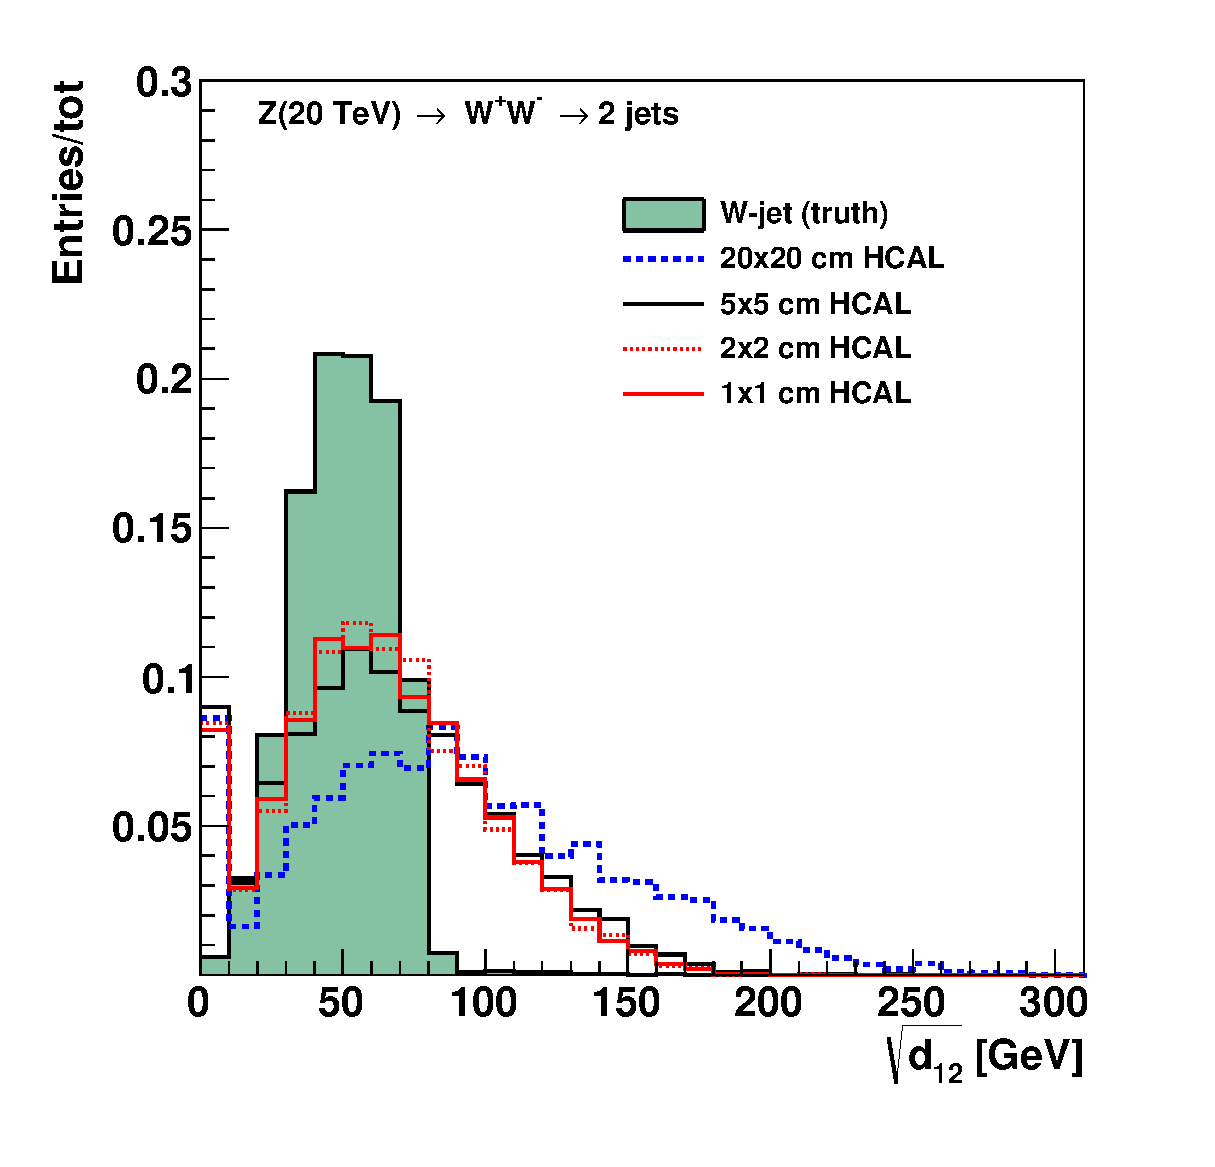
\includegraphics[width=0.43\textwidth]{figs/h20tev_clus_d12_ww1}
   }
   \subfigure[40 TeV] {
   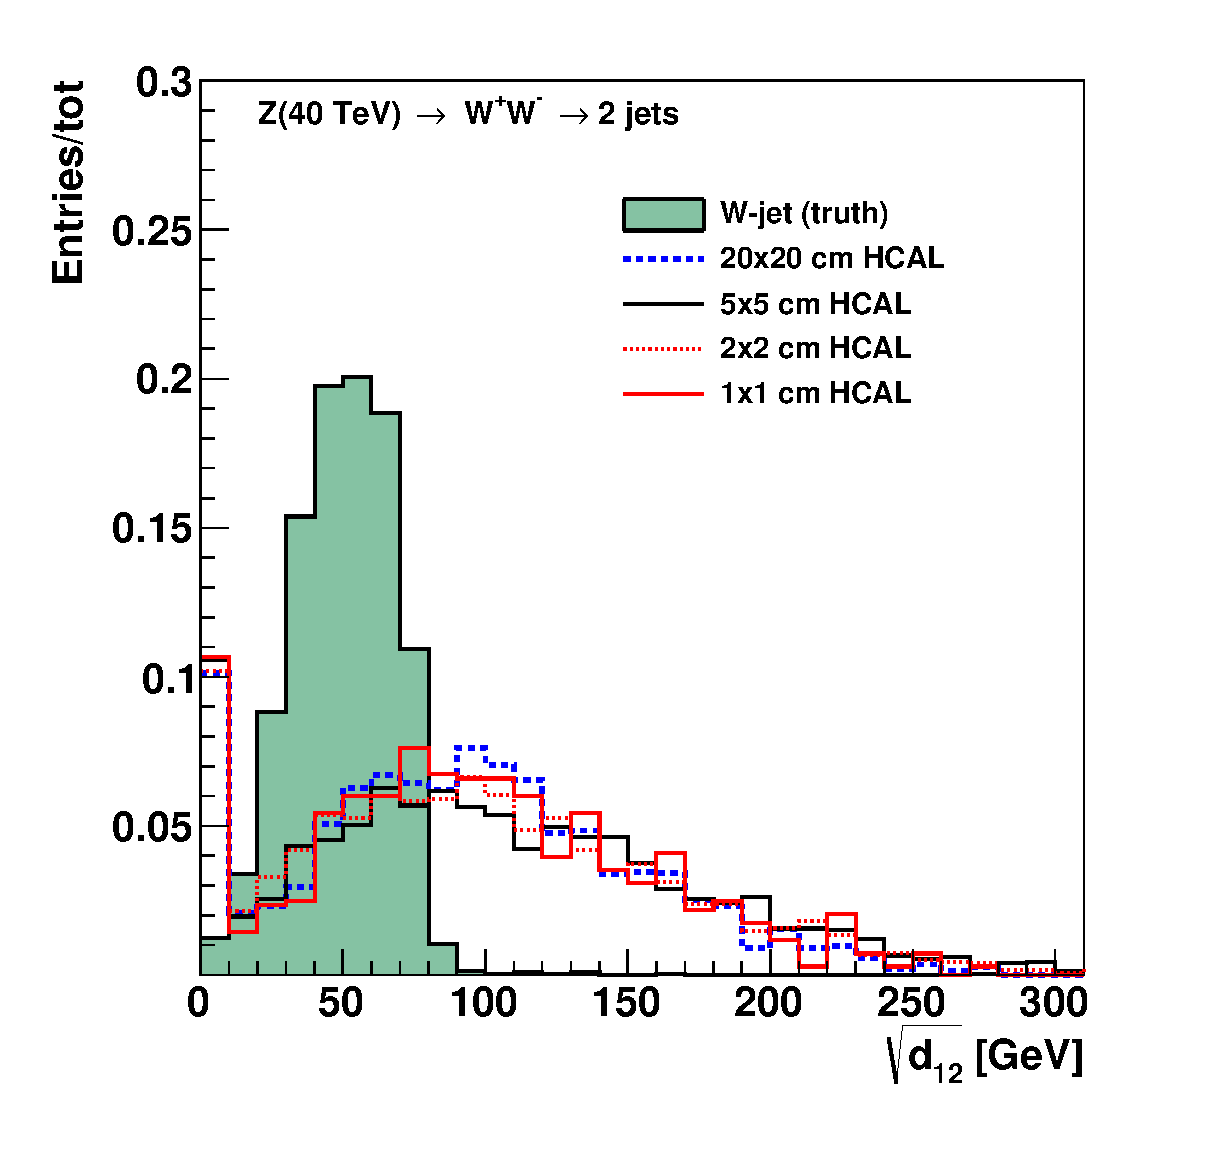
\includegraphics[width=0.43\textwidth]{figs/h40tev_clus_d12_ww1}
   }
\end{center}
\caption{Jet splitting scale for different jet transverse moment and HCAL granularity.}
\label{fig:d12}
\end{figure}




